\subsection{Grafi}
Il problema che intendiamo affrontare in questo elaborato è descritto naturalmente con il formalismo della teoria dei grafi. In questa sezione presentiamo un sottoinsieme minimale di definizioni e risultati che ci consentirà di introdurre e trattare la questione in modo appropriato.

\subsubsection{Definizione e generalità}
Con le premesse viste nella Sezione \ref{subsec:binrel} possiamo definire un \emph{grafo} come segue:
\begin{definition}
    Sia $V$ un insieme finito non vuoto. Sia $E$ una relazione binaria su $V$. La coppia $G = (V, E)$ è un \emph{grafo diretto} (o \emph{orientato}). Con questa notazione:
    \begin{itemize}
        \item $V$ è l'insieme dei \emph{nodi} (o \emph{vertici});
        \item $E$ è una relazione binaria (in generale non simmetrica) che mette in relazione alcuni dei nodi di $G$.
    \end{itemize}
\end{definition}

\begin{example}
    \begin{figure}[t]
        \centering
        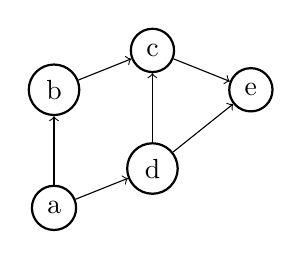
\begin{tikzpicture}[scale=0.5]
            \begin{scope}[every node/.style={circle,thick,draw}]
                \node (a) at (0,0) {a};
                \node (b) at (0,3) {b};
                \node (c) at (2.5,4) {c};
                \node (d) at (2.5,1) {d};
                \node (e) at (5,3) {e};
            \end{scope}

            \begin{scope}
                \path [->] (a) edge node {} (b);
                \path [->] (b) edge node {} (c);
                \path [->] (a) edge node {} (d);
                \path [->] (d) edge node {} (c);
                \path [->] (d) edge node {} (e);
                \path [->] (c) edge node {} (e);
            \end{scope}
            \end{tikzpicture}
        \caption{Rappresentazione grafica di un grafo diretto}
        \label{fig:graph}
    \end{figure}
    Il grafo di Figura \ref{fig:graph} è descritto dalla coppia
    \begin{itemize}
        \item $V = \{a,b,c,d,e\}$
        \item $E = \{(a,b), (a,d), (b,c), (d,c), (c,e), (d,e)\}$
    \end{itemize}
\end{example}

Nel seguito utilizzeremo ampiamente la seguente terminologia:
\begin{definition}
    Sia $G = (V,E)$ un grafo diretto. Consideriamo un arco $(u,v) \in E$. In questo caso $u$ è la \emph{sorgente} dell'arco, mentre $v$ è la \emph{destinazione}. Se il numero di archi uscenti da un nodo è zero tale nodo  è un \emph{pozzo} (dall'inglese \emph{sink}).
\end{definition}

Inoltre adotteremo la seguente notazione per indicare che esiste un arco che collega $a,b \in V$ nel grafo $G = (V,E)$: $\langle a, b \rangle$. Se vi è ambiguità specificheremo la relazione binaria $E$ in pedice: $\langle a, b \rangle_E$.

\subsubsection{Componenti fortemente connesse}
Come abbiamo visto sopra, un grafo diretto è un insieme di elementi (i \emph{nodi}) accoppiato con un insieme di relazioni tra questi elementi (gli \emph{archi}). \accente naturale associare questo concetto all'idea di percorso: ogni grafo è caratterizzato da un insieme di nodi e da uno di \emph{cammini} che consentono di spostarsi da un nodo ad un altro. La seguente definizione sorge in modo spontaneo da questa interpretazione:
\begin{definition}
    Sia $G = (V, E)$ un grafo diretto. Siano $u,v \in V$. Diciamo che $v$ \emph{è raggiungibile} da $u$, o in alternativa \emph{esiste un cammino} da $u$ a $v$, o ancora $\langle u, v \rangle_{E^*}$, se esiste una sequenza finita di nodi $\displaystyle \{x_n\}_{n \in \{0,\dots,K\}}$, tale che $x_0 = u, x_K = v, \langle x_n, x_{n+1} \rangle_E$.
\end{definition}

L'esistenza di un cammino tra nodi fornisce un criterio immediato per partizionare un grafo in gruppi di nodi. Diamo innanzitutto la seguente definizione:
\begin{definition}
    Un grafo diretto $(V,E)$ è \emph{fortemente connesso} se per ogni coppia di nodi $v_1, v_2 \in V$ esiste un cammino da $v_1$ a $v_2$, cioè $\langle v_1, v_2 \rangle_{E^*}$.
\end{definition}

Possiamo individuare i sottografi massimali (cioè la ripartizione del grafo in sottografi che consente di minimizzare il numero di sottografi) fortemente connessi (\hspace*{-0.1cm}\cite[Appendice B]{clrs}):
\begin{definition}
    Le \emph{componenti fortemente connesse} (\emph{strongly connected components}, \emph{SCC}) di un grafo diretto sono i sottografi che compongono la ripartizione (massimale) del grafo in sottografi fortemente connessi.
\end{definition}

\begin{example}
    \begin{figure}[t]
        \centering
        \begin{tikzpicture}[scale=0.5]
            \begin{scope}[every node/.style={circle,thick,draw}]
                \node (a) at (0,0) {a};
                \node (b) at (0,3) {b};
                \node (c) at (2.5,4) {c};
                \node (d) at (2.5,1) {d};
                \node (e)[diamond] at (5,3) {e};
            \end{scope}

            \begin{scope}
                \path [->] (a) edge node {} (b);
                \path [->] (b) edge node {} (c);
                \path [->] (d) edge node {} (a);
                \path [->] (c) edge node {} (d);
                \path [->] (d) edge node {} (e);
                \path [->] (c) edge node {} (e);
            \end{scope}
            \end{tikzpicture}
        \caption{SCC di un grafo diretto}
        \label{fig:graph_cfc_1}
    \end{figure}
    Nel grafo di Figura \ref{fig:graph_cfc_1} le SCC sono rappresentate con forme diverse: $\{a,b,c,d\}, \{e\}$.
\end{example}

Il partizionamento dei nodi in SCC è definito come segue:
\begin{definition} \label{def:scc_partition}
    Sia $G = (V, E)$ un grafo diretto. Il grafo $G^{\superscc} = (V^{\superscc}, E^{\superscc})$, dove:
    \begin{itemize}
        \item $V^{\superscc} = \{C \mid \,C$ è una SCC$\}$;
        \item $E^{\superscc} = \{(A,B) \in V^{\superscc} \times V^{\superscc} \mid A \neq B, \exists m \in A, n \in B, \langle m,n \rangle_E\}$
    \end{itemize}
    è il partizionamento del grafo iniziale in SCC.
\end{definition}

Riportiamo la seguente proprietà immediata:
\begin{proposition}
    Sia $G^{\superscc}$ il grafo delle SCC di un grafo $G$ generico. Allora $G^{\superscc}$ è aciclico.
\end{proposition}
\begin{proof2}
    Supponiamo per assurdo che in $G^{\superscc}$ (i cui nodi sono i sottografi massimali che compongono la partizione delle SCC) esista un ciclo. Allora tutti i nodi di $V^{\superscc}$ facenti parte del ciclo sono mutuamente raggiungibili (percorrendo il ciclo). Quindi tutti i nodi fanno parte della stessa SCC, ma questo è assurdo.
\end{proof2}

\begin{example}
    \begin{figure}[b]
        \centering
        \begin{subfigure}{.45\textwidth}
          \centering
          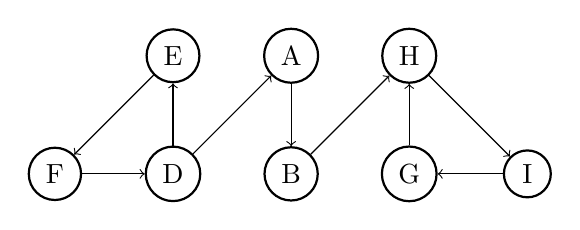
\begin{tikzpicture}[scale=0.5]
            \begin{scope}[every node/.style={circle,thick,draw}]
                \node (A) at (0,3) {A};
                \node (B) at (0,0) {B};

                \node (D) at (-3,0) {D};
                \node (E) at (-3,3) {E};
                \node (F) at (-6,0) {F};

                \node (G) at (3,0) {G};
                \node (H) at (3,3) {H};
                \node (I) at (6,0) {I};
            \end{scope}

            \begin{scope}
                \path [->] (A) edge node {} (B);

                \path [->] (E) edge node {} (F);
                \path [->] (F) edge node {} (D);
                \path [->] (D) edge node {} (E);

                \path [->] (G) edge node {} (H);
                \path [->] (H) edge node {} (I);
                \path [->] (I) edge node {} (G);

                \path [->] (D) edge node {} (A);
                \path [->] (B) edge node {} (H);
            \end{scope}
            \end{tikzpicture}
            \caption{Un grafo diretto}
          \label{fig:graph_cfc_2_graph}
        \end{subfigure}
        \hfill
        \begin{subfigure}{.45\textwidth}
          \centering
          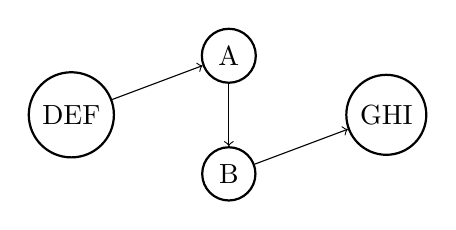
\begin{tikzpicture}[scale=0.5]
            \begin{scope}[every node/.style={circle,thick,draw}]
                \node (A) at (0,3) {A};
                \node (B) at (0,0) {B};

                \node (DEF) at (-4,1.5) {DEF};

                \node (GHI) at (4,1.5) {GHI};
            \end{scope}
                \path [->] (A) edge node {} (B);
                \path [->] (DEF) edge node {} (A);
                \path [->] (B) edge node {} (GHI);
            \begin{scope}

            \end{scope}
            \end{tikzpicture}
            \caption{Grafo delle SCC}
          \label{fig:graph_cfc_2_scc}
        \end{subfigure}
        \caption{Un grafo diretto composto dai nodi $A,B,C,D,E,F,G,H,I$, che possono essere raggruppati nelle SCC $(DEF), (A), (B), (GHI)$.}
    \end{figure}
    Nella Figura \ref{fig:graph_cfc_2_graph} è riportato un grafo diretto generico, nella Figura \ref{fig:graph_cfc_2_scc} si è rappresentato il corrispondente grafo delle componenti fortemente connesse.
\end{example}

Osserviamo infine che la ripartizione in componenti fortemente connesse di un grafo è sempre unica. Per dimostrarlo sfruttiamo il seguente risultato preliminare:
\begin{lemma}
    La relazione binaria $\widehat{E}$ che associa le coppie di nodi mutuamente raggiungibili (si osservi che vale $\widehat{E} \subseteq E^*$) è simmetrica e transitiva.
\end{lemma}
\begin{proof2}
    La simmetria è banale, la transitività discende dal fatto che se $a \widehat{E} b, b \widehat{E} c$, allora è possibile raggiungere $c$ passando per $b$ partendo da $a$, e facendo lo stesso percorso al contrario si dimostra che $a \widehat{E} c$.
\end{proof2}

\begin{corollary}
    La ripartizione in SCC di un grafo è unica.
\end{corollary}
\begin{proof2}
    Supponiamo per assurdo che sia possibile ``scegliere'' se mettere $a,b$ oppure $b,c$ nella stessa SCC, e che questo generi una ripartizione differente. Ma allora si ha anche $a \widehat{E} c$, e quindi un'unico partizionamento.
\end{proof2}

Dato un grafo diretto generico possiamo determinare la partizione delle componenti fortemente connesse utilizzando alcuni algoritmi a complessità lineare \cite{sharir} \cite{tarjan}, che non verranno esposti in questo elaborato.

\subsubsection{Visita in profondità}
Delle due metodologie prevalenti per l'esplorazione di un grafo, \emph{visita in ampiezza} (\emph{Breadth-First-Search}, abbreviato in BFS) e \emph{visita in profondità} (\emph{Depth-First-Search}, abbreviato in DFS), in questo utilizzeremo prevalentemente la seconda. Come dice il nome, questa tecnica consiste nella visita esaustiva di tutti i figli di un nodo, prima di passare agli altri nodi sullo stesso livello.

Riportiamo lo pseudocodice \cite{clrs}, leggermente modificato:\\
\begin{algorithm}[H]
    \label{alg:dfs}
    \KwData{$G = (V,E)$}
    \caption{DFS}
    \SetAlgoLined
    \SetKwProg{Fn}{function}{:}{end}
    \Fn{\textup{dsf-visit}($G = (V,E), n,$ time)}{
        n.color = GRAY\;
        \ForAll{$m \mid (\langle n,m \rangle \land m.$color = WHITE)}{
            time = dfs-visit($G, m,$ time)\;
        }
        n.finishing-time = time\;
        n.color = BLACK\;
        time = time+1\;
        \Return{time}\;
    }
    \Begin{
        \ForAll{$n \in V$}{
            n.color = WHITE\;
        }

        time = 0\;
        \While{$\exists n \in V \mid n.color ==$ WHITE}{
            time = dfs-visit($G,n,$ time)\;
        }
    }
\end{algorithm}
L'attributo \emph{color} dei nodi del grafo consente di distinguere tra quei nodi che sono già stati visitati in modo esauriente (colore nero), quelli per cui è in corso una visita in profondità (colore grigio) e quelli non ancora esaminati dall'algoritmo (colore bianco). Si osservi che la colorazione dei nodi non è solamente accessoria, ma fornisce un meccanismo per evitare un loop infinito nel caso in cui il grafo contenga un ciclo.

Oltre alla colorazione dei nodi, l'algoritmo imposta l'attributo \emph{finishing-time} per ogni nodo, ovvero l'istante di tempo (a partire da \emph{time} $= 0$) in cui è stata terminata la visita esaustiva in profondità per tale nodo. Nello pseudocodice completo vengono considerati altri due attributi: \emph{starting-time} e \emph{parent}. Questi ultimi tre attributi forniscono alcune importanti proprietà all'algoritmo di visita in profondità, che non saranno approfondite in questo lavoro (si vedano \emph{Parenthesis theorem}, \emph{White-path theorem} \cite{clrs}).

L'attributo \emph{finishing-time} è sufficiente per alcune applicazioni che saranno esposte nelle sezioni seguenti.
